\subsection{Sub-Doppler Cooling}
The limit of Doppler cooling is intuitive, it was believed to be the limit of laser cooling until in 1989, the scientists in NIST Gaithersburg reported the measured temperature of ${\rm Na}$ atoms in an optical molasses to be ten times cooler \cite{lett1988observation}. The observation of temperature drastically lower than the theoretical prediction of the Doppler cooling limit surprised scientists and was theoretically explained by Cohen-Tannoudji and collaborators in 1989 \cite{dalibard1989laser}. The temperature in optical molasses is sensitive to laser detuning and polarization, different polarization of light fields drives transition between different $\ket{F,m_F}$ states. To theoretically explain, a two-level system is insufficient and $\ket{F,m_F}$ hyperfine states in atoms' ground state, and the first excited state must be considered.  

\begin{figure}[htbp]
    \centering
    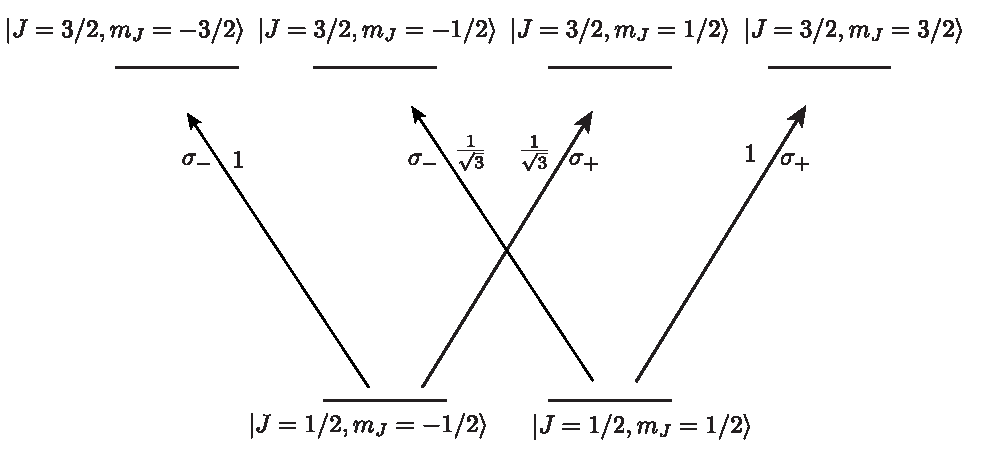
\includegraphics[width=\textwidth]{Chapter2_secs/subDoppler.pdf}
    \caption{Energy levels of ${\rm Na}$ atoms ground state and the first excited state. The Clebsch-Gordon coefficients are labelled for each transition. }
    \label{fig:subDoppler}
\end{figure}

Fig.~(\ref{fig:subDoppler}) shows the energy levels of ${\rm Na}$ atoms ground state and the first excited state. $\sigma_+$ polarized fields couple $\ket{m_J}$ states and $\ket{m_J +1}$ states, $\sigma_-$ polarized fields couples $\ket{m_J}$ states and $\ket{m_J  - 1}$ states. The Clebsch-Gordon coefficients are labeled for each transition. In the optical molasses experiment that observed sub-Doppler limit temperature, the temperature in optical molasses was found to be sensitive to the polarization of light. And in the experiment, three pairs of counter-propagating, crossed linearly polarized laser beams are used. 

The optical field in the lin $\perp$ lin scheme is \cite{metcalf2007laser} 
\begin{align}
    \Vec{E} &= \Vec{E}_0 \hat{x} \cos{\omega t -kz} + \Vec{E}_0 \hat{y} \cos{\omega t +kz}\\
    & = \Vec{E}_0 (\hat{x} + \hat{y})\cos{\omega t}\cos{kz} + \Vec{E}_0 (\hat{x} - \hat{y})\sin{\omega t}\sin{kz}\\
\end{align}

At $z=0$ and $z=\lambda/4$, the atoms are in the linearly polarized field
\begin{equation}
    \Vec{E} =\Vec{E}_0 (\hat{x} \pm \hat{y})\cos{\omega t}
\end{equation}
and  at $z=\lambda/8$, the atoms are in $\sigma_-$ polarized field
\begin{equation}
    \Vec{E} =\Vec{E}_0 \left[\hat{x}\sin{\left(\omega t + \frac{\pi}{4}\right)} - 
        \hat{y}\cos{\left(\omega t + \frac{\pi}{4}\right)}\right].
\end{equation}
At $z=3\lambda/8$, the atoms are in $\sigma_+$ polarized field. The polarization as a function of $z$ is shown in Fig.~(\ref{fig:polarGrad}). 

\begin{figure}[htbp]
    \centering
    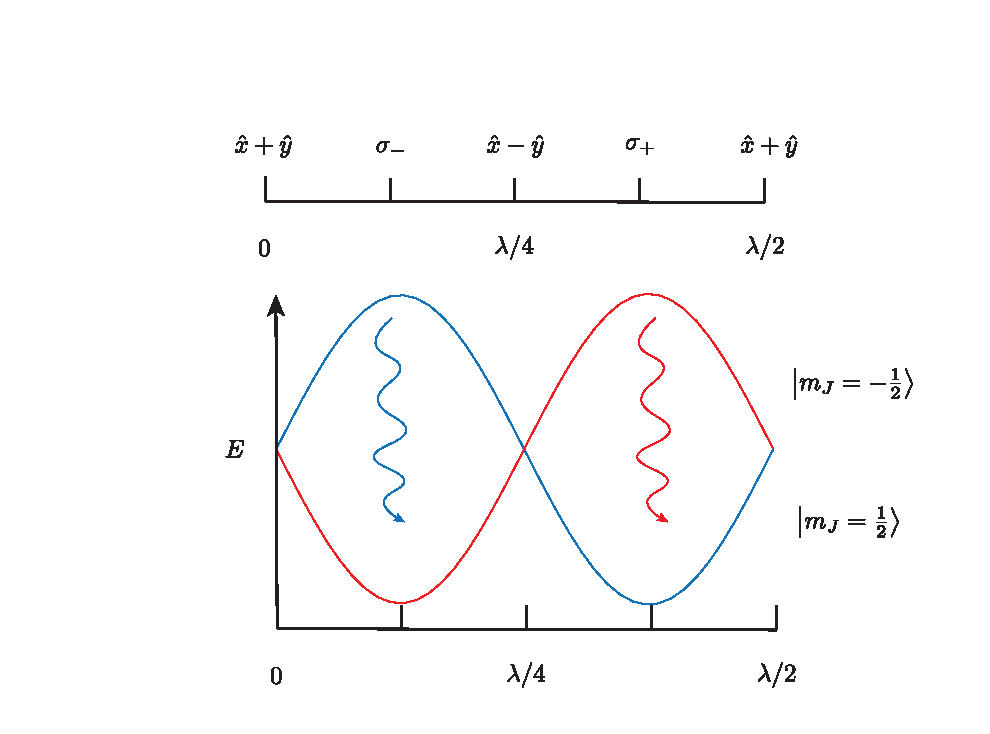
\includegraphics[width=\textwidth]{Chapter2_secs/polarGrad.pdf}
    \caption{The polarization as a function of $z$ in lin $\perp$ lin scheme. }
    \label{fig:polarGrad}
\end{figure}

The polarization is periodic in space in the lin $\perp$ lin scheme, as atoms move, the coupling of $\ket{m_J}$ states changes. When the polarization is $\sigma_+$, $\ket{m_J = -\frac{1}{2}}$ is optically pumped and spontaneously emitted to state $\ket{m_J = \frac{1}{2}}$. And when detuning is large, $|\Omega| \ll \gamma$, the state is in the dressed state of $\ket{m_J = \frac{1}{2}}$. As atoms move, the polarization changes from $\sigma_+$ to $\sigma_-$, and the states transfers from the dressed state of $\ket{m_J = \frac{1}{2}}$ to the dressed state of $\ket{m_J = -\frac{1}{2}}$.

When the detuning is large, the energy of the dressed states is mainly AC Stark shift, 
\begin{align}
    E_{1/2}^{\sigma_+} = -\frac{|\Omega|^2}{\delta}, E_{-1/2}^{\sigma_+} = -\frac{|\Omega|^2}{3\delta}\\\nonumber
    E_{1/2}^{\sigma_-} = -\frac{|\Omega|^2}{3\delta}, E_{-1/2}^{\sigma_-} = -\frac{|\Omega|^2}{\delta}\\\nonumber
\end{align}
The energy is sketched in Fig.~(\ref{fig:polarGrad}) and the difference of denominator originates from the difference in Clebsch-Gordon coefficients between states $\ket{m_J},~\ket{m_J+1}$ and $\ket{m_J},~\ket{m_J-1}$. 

When the atoms move from $\sigma_-$ polarization to $\sigma_+$,  it starts from state $\ket{m_J=-1/2}$ and climbs uphill in potential energy. Along the way, polarization changes gradually, and as it reaches $\sigma_+$ polarization, the state transfers to $\ket{m_J=1/2}$ which has lower potential energy. Then, the climbing process goes on in the periodically polarized field. When the atoms climb uphill it converts kinetic energy to potential energy and slows down. As polarization flips, the energy loss in the state transfer goes to the optical field because the state absorbs lower energy photons and emits higher energy photons in the spontaneous emission process. The technique is also named "Sisyphus cooling", in the Greek mythology, Sisyphus was doomed to roll a stone up a mountain only to have it roll down again.

The limit of Sisyphus cooling was found to be associated with the photon recoil momentum $\hbar k$ and in the early experiments, the temperature of atoms in Optical molasses was measured to be an order of magnitude smaller than the limit of Doppler cooling.
